\documentclass[12pt, a4paper]{article}
\usepackage{enumitem}
\usepackage[left=2cm, right=2cm, top=2cm, bottom=2cm]{geometry}
\usepackage{graphicx}
\usepackage{minted}
\usepackage{xeCJK}

\renewcommand\arraystretch{1.1}
\setCJKmainfont[AutoFakeBold=1.5]{新細明體}

\setminted{
  fontsize=\footnotesize,
  frame=single,
}

\title{
  \vspace{-1cm}
  Systems Programming (2024 Fall)\\
  Handwritten Assignment 1
}
\author{\Large B12902110 呂承諺}
\date{}

\begin{document}
  \maketitle
  \begin{enumerate}
    \item No. If the current working directory is the root directory (\texttt{/}),
    then directories dot (\texttt{.}) and dot-dot (\texttt{..}) both refer to
    the root directory itself.

    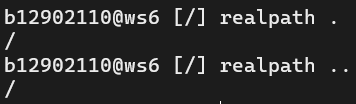
\includegraphics[width=0.4\linewidth]{1_realpath.png}

    \item You can use \verb|lseek| to read from anywhere, but cannot replace existing
    data in the file, because if the file is opened with the \verb|O_APPEND| flag, the
    file offset is set to the end of file before each \verb|write|.

    \inputminted[label=\footnotesize2\_append.c]{c}{2_append.c}
    \inputminted[label=\footnotesize2\_append.txt]{text}{2_append.txt}

    \item Yes, the test is necessary. We can see from the three \verb|dup()| calls that
    the code wants to keep file descriptors \verb|0|, \verb|1|, and \verb|2| open and pointed
    to the same file. However, if the test isn't performed, and \verb|fd| is one of \verb|0|,
    \verb|1|, or \verb|2|, then it would be closed unintentionally.
  \end{enumerate}
\end{document}
